%%%%%%%%%%%%%%%%%%%%%%%%%%%%%%%%%%%%%%%%%
% Short Sectioned Assignment LaTeX Template Version 1.0 (5/5/12)
% This template has been downloaded from: http://www.LaTeXTemplates.com
% Original author:  Frits Wenneker (http://www.howtotex.com)
% License: CC BY-NC-SA 3.0 (http://creativecommons.org/licenses/by-nc-sa/3.0/)
%%%%%%%%%%%%%%%%%%%%%%%%%%%%%%%%%%%%%%%%%

% \documentclass[paper=a4, fontsize=11pt]{scrartcl} % A4 paper and 11pt font size
\documentclass[11pt, a4paper]{book}
\usepackage[T1]{fontenc} % Use 8-bit encoding that has 256 glyphs
\usepackage[utf8]{inputenc}
\usepackage{fourier} % Use the Adobe Utopia font for the document - comment this line to return to the LaTeX default
\usepackage{listings} % para insertar código con formato similar al editor
\usepackage[spanish, es-tabla]{babel} % Selecciona el español para palabras introducidas automáticamente, p.ej. "septiembre" en la fecha y especifica que se use la palabra Tabla en vez de Cuadro
\usepackage{url} % ,href} %para incluir URLs e hipervínculos dentro del texto (aunque hay que instalar href)
\usepackage{graphics,graphicx, float} %para incluir imágenes y colocarlas
\usepackage[gen]{eurosym} %para incluir el símbolo del euro
\usepackage{cite} %para incluir citas del archivo <nombre>.bib
\usepackage{enumerate}
\usepackage{hyperref}
\usepackage{graphicx}
\usepackage{tabularx}
\usepackage{booktabs}

\usepackage[table,xcdraw]{xcolor}
\hypersetup{
	colorlinks=true,	% false: boxed links; true: colored links
	linkcolor=black,	% color of internal links
	urlcolor=cyan		% color of external links
}
\renewcommand{\familydefault}{\sfdefault}
\usepackage{fancyhdr} % Custom headers and footers
\pagestyle{fancyplain} % Makes all pages in the document conform to the custom headers and footers
\fancyhead[L]{} % Empty left header
\fancyhead[C]{} % Empty center header
\fancyhead[R]{Gestión de ofertas publicadas en canales de Discord y Telegram} % My name
\fancyfoot[L]{} % Empty left footer
\fancyfoot[C]{} % Empty center footer
\fancyfoot[R]{\thepage} % Page numbering for right footer
%\renewcommand{\headrulewidth}{0pt} % Remove header underlines
\renewcommand{\footrulewidth}{0pt} % Remove footer underlines
\setlength{\headheight}{13.6pt} % Customize the height of the header

\usepackage{titlesec, blindtext, color}
\definecolor{gray75}{gray}{0.75}
\newcommand{\hsp}{\hspace{20pt}}
\titleformat{\chapter}[hang]{\Huge\bfseries}{\thechapter\hsp\textcolor{gray75}{|}\hsp}{0pt}{\Huge\bfseries}
\setcounter{secnumdepth}{4}
\usepackage[Lenny]{fncychap}


\begin{document}

	% Plantilla portada UGR
	\begin{titlepage}
\newlength{\centeroffset}
\setlength{\centeroffset}{-0.5\oddsidemargin}
\addtolength{\centeroffset}{0.5\evensidemargin}
\thispagestyle{empty}

\noindent\hspace*{\centeroffset}\begin{minipage}{\textwidth}

\centering

\includegraphics[width=0.9\textwidth]{logos/logo_ugr.jpg}\\[1.4cm]

\textsc{ \Large TRABAJO FIN DE GRADO\\[0.2cm]}
\textsc{ GRADO EN INGENIERÍA INFORMÁTICA}\\[1cm]

{\Huge\bfseries Título \\}
\noindent\rule[-1ex]{\textwidth}{3pt}\\[3.5ex]
{\large\bfseries Subtítulo }
\end{minipage}

\vspace{2.5cm}
\noindent\hspace*{\centeroffset}
\begin{minipage}{\textwidth}
\centering

\textbf{Autor}\\ {Jerónimo Chaves Caballero}\\[2.5ex]
\textbf{Director}\\ {Juan Julián Merelo Guervós}\\[2cm]

\includegraphics[width=0.3\textwidth]{logos/etsiit_logo.png}\\[0.1cm]
\textsc{Escuela Técnica Superior de Ingenierías Informática y de Telecomunicación}\\
\textsc{---}\\
Granada, Junio de 2023
\end{minipage}
\end{titlepage}


	% Plantilla prefacio UGR
	\thispagestyle{empty}

\begin{center}
{\large\bfseries Título \\ Subtítulo }\\	%FIXME: Cambiar Título / Subtítulo cuando lo tengamos
\end{center}
\begin{center}
Jerónimo Chaves Caballero\\
\end{center}

%\vspace{0.7cm}

\vspace{0.5cm}
\noindent\textbf{Palabras clave}: \textit{software libre}
\vspace{0.7cm}

\noindent\textbf{Resumen}
	

\cleardoublepage

\begin{center}
	{\large\bfseries Same, but in English}\\	%FIXME: Cambiar contenido por el Título / Subtítulo en inglés
\end{center}
\begin{center}
	Jerónimo Chaves Caballero\\
\end{center}
\vspace{0.5cm}
\noindent\textbf{Keywords}: \textit{open source}, \textit{floss}
\vspace{0.7cm}

\noindent\textbf{Abstract}


\cleardoublepage

\thispagestyle{empty}

\noindent\rule[-1ex]{\textwidth}{2pt}[4.5ex]

D. \textbf{Juan Julián Merelo Guervós}, Profesor del  departamento de Ingeniería de Computadores, Automática y Robótica.

\vspace{0.5cm}

\textbf{Informo:}

\vspace{0.5cm}

Que el presente trabajo, titulado \textit{\textbf{Chief}},	%FIXME: Cambiar 'Chief' por el título definitivo del trabajo
ha sido realizado bajo mi supervisión por \textbf{Jerónimo Chaves Caballero}, y autorizo la defensa de dicho trabajo ante el tribunal
que corresponda.

\vspace{0.5cm}

Y para que conste, expiden y firman el presente informe en Granada a Junio de 2023.

\vspace{1cm}

\textbf{El/la director(a)/es: }

\vspace{5cm}

\noindent \textbf{(Juan Julián Merelo Guervós)}

\chapter*{Agradecimientos}






	% Índice de contenidos
	\newpage
	\tableofcontents

	% Índice de imágenes y tablas
	\newpage
	\listoffigures

	% Si hay suficientes se incluirá dicho índice
	\listoftables 
	\newpage

	\chapter{Introducción}

Este proyecto es software libre, y está liberado con la licencia GPL 3\cite{gplv3}.

La intención de este proyecto es solucionar el siguiente problema:

\textbf{Resumir las ofertas de un canal de Telegram o Discord en los precios actuales y el mínimo alcanzado para un videojuego.}

En nuestro caso, estamos basándonos sobre todo en uno de los canales más utilizados para este tipo de problema: el canal Ofertas Juegos en Telegram.

Teniendo esto en cuenta, debemos de encontrar una solución adecuada para esto que sea rápida de desarrollar, pero fácilmente escalable en
caso de que queramos partir de esta base para crear algo más grande.


	\chapter{Estado del arte}

Como se ha mencionado anteriormente, hay bastantes maneras de buscar ofertas de 
videojuegos, ya sea por portales web como \url{chollometro.com}, o por canales de 
comunicación, teniendo como ejemplo específico a \url{ofertasjuegos.es} en lo que 
respecta a canales de Telegram.

Es cierto que podemos buscar ofertas en ambos métodos (sobre todo en el ejemplo 
puesto para portales web dedicados a ello), pero aun así no podemos saber cuándo 
hay una oferta de algo que nos interesa al momento si no estamos revisando todo el 
rato el portal web, o puede que se pierda en todos los mensajes que se envían en el 
canal de Telegram.

Es por esto que este proyecto pretende coleccionar las ofertas desde un mismo sitio 
para que sea fácil explorar por ellas, buscando específicamente lo que nos interesa 
y sin la necesidad de pasar por todas esas ofertas que son irrelevantes para 
nosotros.

Esto ayuda a que el usuario pueda centrarse solamente en un único sitio y no tener 
la necesidad de estar entrando en varios portales web o canales de Telegram para 
encontrar ofertas.

Para el desarrollo del proyecto, necesitamos obtener la información de los 
distintos sitios de ofertas. En este caso, vamos a centrarnos primero en obtener 
los datos desde Telegram, que cuenta con una API para poder obtener los mensajes de 
un canal o chat, además de su uso extendido para los famosos bots de la aplicación.

Por tanto, es fácil encontrar librerías que permiten utilizar la API de Telegram de  
una manera más sencilla. Dentro de la propia documentación de Telegram 
podemos encontrar una lista curada 
\footnote{Bot API Library Examples \url{https://core.telegram.org/bots/samples}} de 
los que tienen más librerías.

Teniendo esto en cuenta, vamos a categorizar los lenguajes para elegir la mejor 
opción para el proyecto.

Las categorías serían:

\begin{itemize}
    \item \textbf{Facilidad de aprendizaje/entendimiento}: Queremos un lenguaje que 
    si no lo conocemos, podamos adaptarnos rápidamente a él.
    \item \textbf{Comunidad}: Si contamos no solamente que el lenguaje sea de
    rápida adaptación, sino que además tenga una comunidad extensa, nos será más 
    fácil resolver nuestras dudas.
    \item \textbf{Eficiencia del lenguaje}: Además de los puntos anteriores, es 
    importante elegir un lenguaje que sea eficiente en cuanto a recursos, ya que 
    podemos encontrarnos con que consuma demasiada memoria o haga que nuestra 
    factura sea un poco más alta de lo que esperábamos. Esto ya se ha explorado y 
    se puede encontrar una lista curada \cite{eficiencia} de los lenguajes.
\end{itemize}

Teniendo en cuenta estas categorías y la lista que nos proporcionan en la 
documentación de Telegram, hemos decidido utilizar Go como lenguaje de programación 
para nuestro proyecto.
	
	\chapter{Planificación}

La planificación de un proyecto llega a ser una de las partes más cruciales del 
desarrollo de este y de su éxito. Es el proceso mediante el cual se definen los 
objetivos, se establecen las tareas y se asignan los recursos necesarios para 
llevar a cabo la creación de un software de manera eficiente y efectiva.

En este capítulo vamos a exponer las distintas metodologías que 
vamos a utilizar tanto para las tareas como para el desarrollo además de dónde se 
puede encontrar el repositorio y las herramientas utilizadas para seguir las 
metodologías.

\section{Metodologías utilizadas}

Decidiendo las distintas metodologías que queremos seguir durante el proyecto, se 
han seleccionado tres metodologías que se llegan a usar en el desarrollo ágil: 
\textbf{Kanban}, \textbf{Desarrollo Dirigido por Pruebas} e \textbf{Integración 
Continua}.

Primero, \textbf{Kanban} \cite{kanban} es una metodología de desarrollo ágil que se 
emplea para visualizar y gestionar el flujo de trabajo de un proyecto, basándose en 
tres tableros: tareas pendientes, en progreso y completadas. Las distintas tareas 
se representan en tarjetas, que vamos moviendo de un tablero a otro según el estado 
de estas.

Nosotros hemos añadido un cuarto tablero, donde pondremos que tareas están 
bloqueadas por otra tarea o proceso. Así, vemos de un vistazo que debemos de 
priorizar para que el proyecto avance (figura \ref{fig:tabla-kanban}).

\begin{figure}[h]
    \centering
    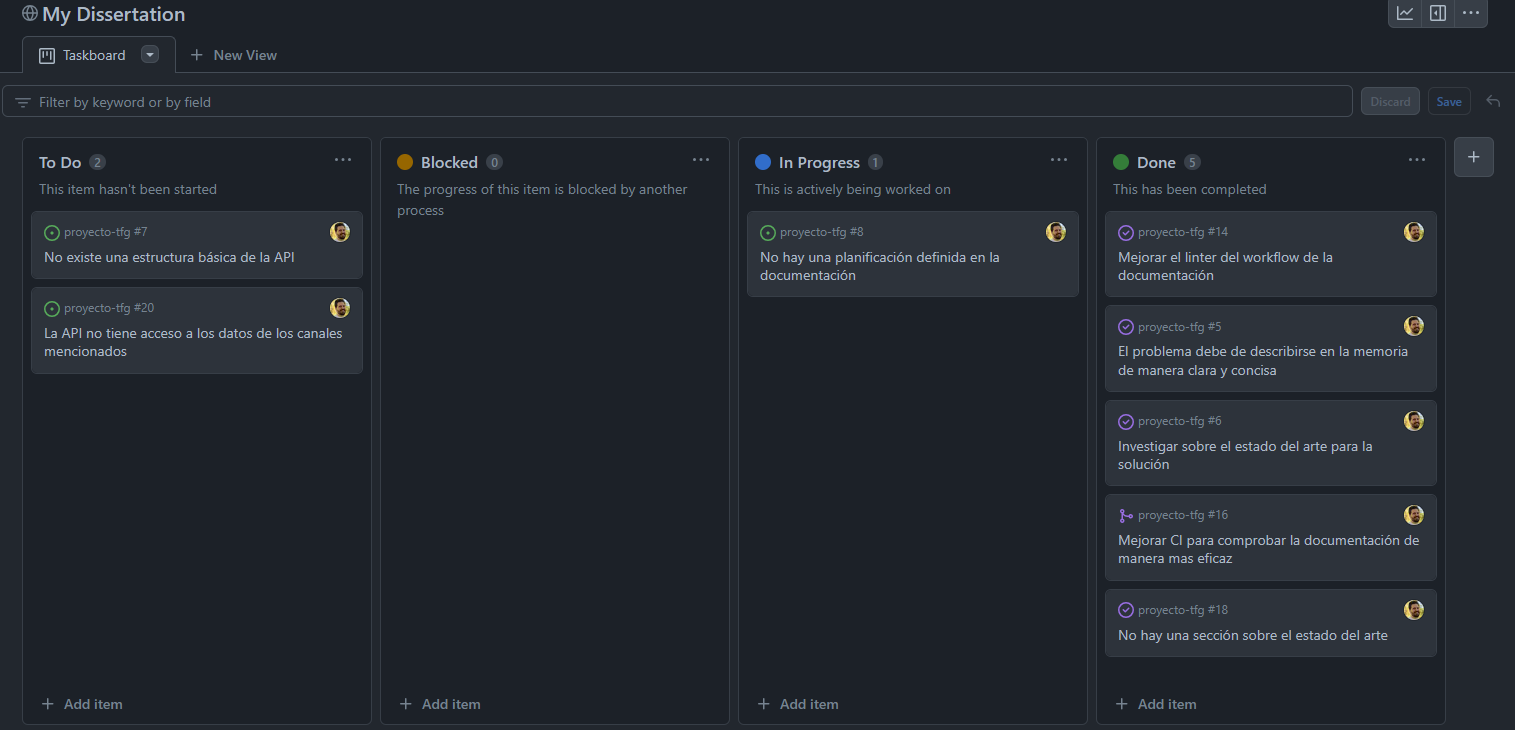
\includegraphics[scale=0.3]{figuras/github-projects-proyecto-tfg.png}
    \caption{Tablas Kanban dentro de GitHub Projects.}
    \label{fig:tabla-kanban}
\end{figure}

El \textbf{Desarrollo Dirigido por Pruebas} (\textbf{TDD}, en inglés \textbf{Test 
Driven Development}) \cite{tdd} es una práctica de desarrollo de software que se 
basa en crear primero las pruebas antes de implementar el código de la 
funcionalidad. Con esto, podemos conseguir tener el código más limpio y que se 
compruebe de manera fácil que el código funciona como indican los requisitos.

Por último, la \textbf{integración continua} (\textbf{CI}, en inglés 
\textbf{Continuous Integration}) \cite{ci} es una metodología de desarrollo de 
software que consiste en integrar los nuevos cambios en el código verificando 
previamente que estos cambios no rompen el código existente. Para llegar a esto, se 
aplicará lo siguiente:

\begin{enumerate}
    \item \textbf{Automatización de pruebas}: Las pruebas (que hemos mencionado 
    anteriormente) serán automatizadas en el flujo de trabajo.
    \item \textbf{Compilación automatizada}: Se compilará el código con los cambios 
    realizados para revisar que no hay problemas durante la compilación.
    \item \textbf{Despliegue automatizado}: Se desplegará el código en un entorno 
    para su acceso en el momento en el que lleguemos al producto mínimo viable.
\end{enumerate}

\section{Usuarios}

Para el desarrollo de este proyecto, se han definido los siguientes tipos de 
usuarios:

\begin{itemize}
    \item \textbf{Tribunal de evaluación}: Este trabajo de fin de grado será 
    evaluado por un grupo de profesores de la universidad y, por tanto, se debe de 
    asociar una memoria que contenga la explicación del proyecto.
    \item \textbf{Estudiante}: Cuenta con un presupuesto limitado. Puede preferir 
    comprar un mayor número de videojuegos con ese presupuesto o bien, comprar por 
    el que más interesado está a un precio menor de su precio de venta al público 
    (PVP) para ahorrar dinero.
    \item \textbf{Coleccionista}: El presupuesto es más elevado que el anterior 
    caso que hemos descrito. Le interesa más la disponibilidad de los videojuegos, 
    aunque también aprecia poder llevárselo por un precio menor.
\end{itemize}

\section{Historias de usuario}

Habiendo identificado los distintos usuarios que hemos encontrado, podemos 
desarrollar las historias de usuario relacionadas o casos de uso que se pueden 
desarrollar para este proyecto. Para ello, hemos definido las siguientes historias:

\subsection{[HU00] Generar una buena estructura en la memoria}

Como tribunal de TFG, necesito entender todos los términos que figuran en el TFG, 
entender claramente cuál es la aportación del estudiante, y los retos que ha 
superado. Y quiero verlo por escrito en un informe que esté correctamente escrito, 
tenga el formato correcto, y exprese claramente el trabajo realizado.

\textbf{Condiciones de satisfacción}:

\begin{itemize}
    \item La memoria debe de estar fácilmente accesible.
    \item La memoria debe de contener un estudio acerca del estado del arte.
    \item La memoria debe de contener información acerca de la metodología que se 
    esté utilizando.
    \item La memoria debe de contener la definición de los objetivos e historias de 
    usuario del proyecto.
    \item La memoria debe de estar correctamente escrita.
\end{itemize}

\subsection{[HU01] Buscar videojuegos por nombre}

Como estudiante/coleccionista, quiero poder buscar un videojuego por su nombre para 
obtener las distintas tiendas que lo venden y su precio, además de su enlace de 
compra para cada una.

Como tribunal de TFG, quiero conocer el desarrollo de la solución necesario para 
poder obtener la información de un videojuego por su nombre, para así poder 
evaluar al estudiante.

\textbf{Condiciones de satisfacción}:

\begin{itemize}
    \item La solución debe de poder buscar un videojuego por su nombre.
    \item La solución debe de poder obtener las distintas tiendas que venden el 
    videojuego.
    \item La solución debe de poder obtener el precio de cada tienda.
    \item La solución debe de poder obtener el enlace de compra del videojuego para 
    cada tienda.
    \item El desarrollo de la solución debe de estar correctamente explicado, tanto 
    la parte de desarrollo con código como las necesidades para implementarlo.
\end{itemize}

\section{Seguimiento del desarrollo}

Para el seguimiento del desarrollo del proyecto, hemos decidido usar Git como 
sistema de control de versiones y la plataforma GitHub para alojar el repositorio 
remoto del proyecto.

Lo bueno de GitHub es que, además, nos ofrece más herramientas para seguir las 
distintas metodologías que hemos mencionado anteriormente:

\begin{itemize}
    \item \textbf{GitHub Issues}: Con Issues podemos añadir nuestras tareas para el 
    proyecto para poder saber que hace falta llevar a cabo.
    \item \textbf{GitHub Milestones}: Con Milestones podemos agrupar las tareas que 
    hemos ido creando poco a poco y priorizar lo que se debe de hacer antes. 
    Además, con esto hemos podido adecuar un Producto Mínimo Viable (MVP en inglés) 
    con la Milestone 1. Si se quiere ver los distintos Milestones, se puede 
    mediante el siguiente enlace: 
    \url{https://github.com/jero-dev/proyecto-tfg/milestones}
    \item \textbf{GitHub Projects}: Con Projects podemos generar un tablero para 
    seguir la metodología Kanban y comprobar el estado de las tareas o issues que 
    están representadas por las tarjetas (figura \ref{fig:tabla-kanban}). El 
    proyecto se puede encontrar en el siguiente enlace: 
    \url{https://github.com/users/jero-dev/projects/1}
    \item \textbf{GitHub Actions}: Gracias a esta herramienta podemos automatizar 
    tanto la compilación como la ejecución de pruebas cada vez que se añadan 
    cambios. Por tanto, gracias a esto, podemos seguir la metodología de 
    integración continua durante el desarrollo.
\end{itemize}


	\chapter{Implementación}

Ya teniendo todo planificado y sabiendo que metodologías vamos a seguir, 
empezaremos con la implementación de la solución. Lo primero, por supuesto, es 
haber creado nuestro \href{https://github.com/jero-dev/proyecto-tfg}
{repositorio en GitHub} donde subir todos los progresos que hagamos no solamente en 
el propio desarrollo de la solución, sino también en la redacción de la memoria del 
trabajo.

En cuanto a los otros elementos que hemos mencionado como las 
\href{https://github.com/jero-dev/proyecto-tfg/issues}{issues}, los 
\href{https://github.com/jero-dev/proyecto-tfg/milestones}{milestones} y 
\href{https://github.com/users/jero-dev/projects/1}{nuestro tablero Kanban}, se 
pueden encontrar en los enlaces que se encuentran en este párrafo.

Con todo esto ya realizado, es momento de empezar a identificar las historias de 
usuario que podemos encontrar gracias a la definición de personas que llegamos a 
realizar en el capítulo de introducción.

\section{Historias de usuario}

Habiendo identificado los distintos usuarios que hemos encontrado, podemos 
desarrollar las historias de usuario relacionadas o casos de uso que se pueden 
desarrollar para este proyecto. Para ello, hemos definido las siguientes historias:

\subsection{[HU01] Buscar videojuegos por nombre}

Como persona menor de 20 años/coleccionista, quiero poder buscar un videojuego por 
su nombre para obtener las distintas tiendas que lo venden y su precio, además de 
su enlace de compra para cada una.

\textbf{Condiciones de satisfacción}:

\begin{itemize}
    \item La solución debe de poder buscar un videojuego por su nombre.
    \item La solución debe de poder obtener las distintas tiendas que venden el 
    videojuego.
    \item La solución debe de poder obtener el precio de cada tienda.
    \item La solución debe de poder obtener el enlace de compra del videojuego para 
    cada tienda.
\end{itemize}

\subsection{[HU02] Obtener avisos automáticos acerca de un videojuego}

Como coleccionista, tendría en cuenta la opción de obtener avisos automáticos de la 
disponibilidad de un videojuego en concreto en el que tengo interés.

\textbf{Condiciones de satisfacción}:

\begin{itemize}
    \item La solución debe de ofrecer avisos automáticos de la disponibilidad de un 
    videojuego.
    \item En el aviso debe de aparecer el precio de cada tienda.
    \item En el aviso debe de aparecer el enlace de compra del videojuego para 
    cada tienda.
\end{itemize}

En nuestro caso nos centraremos principalmente en la primera historia de usuario, 
completando la segunda en caso de que tengamos tiempo suficiente para ello.

\section{Diseño de la aplicación}

Teniendo ya las historias de usuario, vamos a empezar a diseñar la solución. Para 
ello, seguiremos el diseño dirigido por dominios (en inglés, Domain Driven Design o 
DDD) \cite{ddd} para identificar de manera correcta el dominio del problema y poder 
así concentrarnos totalmente en él.

\begin{itemize}
    \item \textbf{Dominio del problema:} Tenemos como dominio del problema la 
    gestión de ofertas y promociones de productos (aunque nos centremos en 
    videojuegos). En cuanto a los conceptos (entidades) que hemos identificado, 
    tenemos solamente uno: el de \textbf{videojuego}. Aparte, tenemos también un 
    ``value object'' que sería el de \textbf{oferta} y un agregado de ambos que es 
    el de \textbf{producto}.
    \begin{itemize}
        \item \textbf{Videojuego}: Las propiedades de esta entidad serían un 
        \textbf{identificador único}, el \textbf{nombre} del producto y la 
        \textbf{plataforma} en la que se juega.
        \item \textbf{Oferta}: Las propiedades de este ``value object'' serían el 
        \textbf{precio} y el \textbf{enlace} a la tienda donde se encuentra la 
        oferta.
        \item \textbf{Producto}: Las propiedades de este agregado serían un 
        \textbf{videojuego} y una \textbf{lista de ofertas} que se han encontrado 
        para este.
    \end{itemize}
    \item \textbf{Contexto delimitado:} Para centrarnos en el problema, tenemos que 
    delimitar el contexto del mismo. Aquí tenemos claro que el contexto es la 
    gestión de ofertas.
    \item \textbf{Servicios de dominio:} Los servicios de dominio encapsulan la 
    lógica de negocio que no pertenece a ninguna entidad o valor. Aquí podemos 
    encontrar dos claros servicios de dominio: el procesamiento de los mensajes y 
    la gestión de las ofertas.
\end{itemize}

Teniendo el análisis realizado, podemos plasmarlo directamente a la estructura de 
nuestra aplicación. Primero, crearemos un directorio llamado \verb|entity| donde 
guardaremos la entidad \verb|VideoGame| con las propiedades mencionadas. Después, 
añadimos otro directorio llamado \verb|value_object| donde guardaremos el ``value 
object'' de \verb|Offer| también con sus propiedades apropiadas.

Este tipo de datos son básicos, sin ningún tipo de método fuera de un constructor y 
dos métodos de acceso para las propiedades de \verb|Offer|. Por ello, no vamos a 
tener pruebas unitarias para ellos.

Siguiendo con los conceptos que hemos identificado, queda el agregado de 
\verb|Product|. Este va a estar contenido en otro directorio llamado 
\verb|aggregate| en el que encontraremos tanto el tipo \verb|Product| como también 
las pruebas unitarias para el mismo en dos ficheros: \verb|product.go| y 
\verb|product_test.go|.

Necesitaremos guardar estos datos de alguna manera, así que añadiremos otro 
directorio llamado \verb|domain| que contendrá otro llamado \verb|product|. Aquí 
tendremos una interfaz que será la responsable de crear el contrato de cómo se debe 
de comportar un repositorio (por ello llamaremos al fichero \verb|repository.go|) 
para que no tengamos que depender de una tecnología en concreto. 

Para tener nuestro producto mínimamente viable, generaremos primero un repositorio 
en memoria que, si finalmente tenemos tiempo, podremos cambiar por uno que se 
conecte a una base de datos de nuestra preferencia. Con ello, tendremos otro  
directorio llamado \verb|memory| con dos ficheros: \verb|memory.go| y su respectivo 
fichero de pruebas unitarias \verb|memory_test.go|.

Finalmente, llegamos a los servicios de dominio. Añadimos un directorio llamado 
\verb|service| que contendrá los distintos casos de uso o servicios. Uno se llamará 
\verb|offer_manager.go| y otro será \verb|message_processor.go|. Al ser una lógica 
más compleja, dejaremos la implementación de estos para la siguiente sección. 
También añadiremos el fichero principal de esta aplicación que llamaremos 
\verb|api.go|, ya que es lo que al final será esta aplicación: una API.

\section{Procesamiento de mensajes}

Como hemos mencionado, el servicio de procesamiento de mensajes tiene una lógica 
más compleja, por el hecho de que tiene que encontrar el videojuego que se 
encuentra en el mensaje junto con la oferta mencionada en el mismo. Primero de 
todo, necesitamos ver cómo es el tipo de mensajes que se encuentran en los canales 
de ofertas. En la figura \ref{fig:ejemplo de oferta} se puede ver uno de los 
mensajes de los principales canales de ofertas:

\begin{figure}[h]
    \centering
    
\includegraphics[scale=0.5]{figuras/ejemplo-ofertasjuegos.png}
    \caption{Ejemplo de una notificación de oferta.}
    \label{fig:ejemplo de oferta}
\end{figure}

La mayoría de mensajes que se encuentran en los canales de ofertas tienen el mismo 
formato, así que podemos aprovechar esta característica para llegar a procesarlos 
con una expresión regular.

Dentro del fichero \verb|message_processor.go| crearemos una interfaz llamada 
\verb|MessageProcessor| que declarará solamente un método público que hará la 
interpretación de datos: \verb|ParseMessage|. Este método recibirá el mensaje y 
devolverá el nombre del videojuego, la plataforma, el precio y el enlace de compra.

Para ello, implementaremos el método dentro de una estructura que siga el contrato 
de la interfaz. Esta estructura se llamará \verb|MessageProcessorService| que 
implementará la interfaz mencionada. En el método utilizaremos tres expresiones 
regulares para encontrar los campos:

\begin{itemize}
    \item \verb|gameRegex|: Esta expresión regular busca un patrón que comienza 
    con un emoji de flecha hacia abajo, seguido de un conjunto de caracteres que no 
    contienen '\#', luego '\#', y finalmente, una cadena de caracteres de palabra 
    (letras, dígitos o guiones bajos) después de '\#'.
    \item \verb|priceRegex|: Esta expresión regular busca la presencia de 
    ``BAJONAZO'' o ``FLASH'' seguido de un precio expresado en euros.
    \item \verb|linkRegex|: Esta expresión regular busca cualquier URL que comience 
    con 'http://' o 'https://', seguido de cualquier secuencia de caracteres no 
    espaciados.
\end{itemize}

Esta implementación se ha hecho y comprobado gracias a haber realizado las pruebas 
unitarias desde el principio, utilizando un grupo de nueve casos de prueba para que 
el método funcione como se espera. Estos nueve casos son mensajes reales que se han 
encontrado en el canal de \href{https://ofertasjuegos.es/}{Ofertas Juegos}, uno de 
los grupos de canales más populares de ofertas de videojuegos en Telegram.

En cuanto a por qué hemos creado una interfaz para este servicio, es por el hecho 
de que en el futuro nos ayudará para crear pruebas unitarias de manera más 
sencilla, pero eso lo veremos en la siguiente sección.

\section{Gestión de ofertas}

Ya con la lógica de procesamiento de mensajes implementada, pasamos al otro 
servicio de dominio, que es el de gestión de ofertas. Este servicio se encargará de 
tanto añadir una oferta como de obtener las ofertas de un título en concreto en 
todas las plataformas.

Primero de todo, seguiremos la misma estrategia de generar primero una interfaz que 
contenga el contrato que será necesario cumplir en el momento de la implementación. 
Esta interfaz se llamará \verb|OfferManager| y tendrá dos métodos: 
\verb|StoreOffer| y \verb|GetGameOffers|. El primero añadirá una oferta a un 
producto, mientras que el segundo devolverá las ofertas de un videojuego en todas 
las plataformas en la que esté disponible.

A la hora de implementar la lógica de \verb|StoreOffer|, debemos de comprobar si el 
producto existe en el repositorio. Si este no existe, se crea y añadiremos la 
oferta que se menciona. Si existe, obtenemos la oferta y la añadimos al producto. 
En el caso de añadir la oferta, se verificaba de por sí si el enlace al producto en 
la tienda en el método \verb|AddOffer| del agregado de producto, y solamente se 
actualiza el precio.

Es por esto que vamos a necesitar un nuevo método en el repositorio para devolver 
el producto que coincide con el nombre y la plataforma que se le pasa como 
parámetros. Para ello, añadimos el método \verb|FindByNameAndPlatform| a la clase 
\verb|ProductRepository|. Por supuesto, se pueden encontrar las pruebas unitarias 
relacionadas en el fichero \verb|memory_test.go|.

Ya con el nuevo método, vamos a implementar el servicio de almacenamiento de 
ofertas. Tendremos un nuevo método llamado \verb|StoreOffer| que recibirá el nombre 
del videojuego, la plataforma de este, el precio de la oferta y el enlace donde 
encontrarla.

Teniendo el almacenamiento de las ofertas, vamos a implementar la devolución de las 
ofertas de un videojuego en todas sus plataformas. Pero, todavía no tenemos otro 
método necesario en la capa de repositorio: necesitamos encontrar las ofertas por 
solamente el nombre del videojuego. Este método se llamará \verb|FindByName|.

Con esto ya hecho, podemos implementar el método \verb|GetGameOffers| que recibirá 
el nombre del videojuego y devolverá las ofertas de este en todas sus plataformas.


	% Presupuesto

	% Conclusiones
	\chapter{Conclusiones y trabajos futuros}

Aún teniendo ya una solución funcional y que cubre las necesidades de los usuarios, 
hemos comentado también que existen otras opciones que finalmente no hemos 
implementado por falta de tiempo, ya sea para desarrollar, investigar o probar.

Es por eso que se puede extraer de varias secciones de implementación algunas 
mejoras que se podrían realizar en el futuro, además de nuevas funcionalidades en 
la solución, ya que también tenemos otra historia de usuario identificada que no 
hemos llegado a implementar por no ser la más prioritaria.

\section{Conclusiones}

En conclusión, hemos conseguido desarrollar una solución que cubre las 
necesidades de los usuarios, que es la obtención de ofertas de manera rápida. Por 
supuesto, hemos identificado mejoras, pero al haber llevado a cabo un diseño de la 
aplicación con DDD, algunas de ellas se podrían efectuar de manera más sencilla que 
si no lo hubiéramos hecho.

El principal reto de este trabajo ha sido sobre todo el procesamiento de los 
mensajes, ya que estos, aunque siguen un patrón finalmente, están escritos en 
lenguaje natural, por lo que posiblemente en cuanto añadamos más canales de 
información, las expresiones regulares que se utilicen varíen.

Aunque no fueran el objetivo principal de este trabajo, también hemos aprendido 
como los bots o apps de servicios de mensajería pueden ser una herramienta muy 
potente no solo para la comunicación, sino también para la automatización o 
integración de servicios.

\section{Trabajos futuros}

Aquí podemos dividir las posibles mejoras en dos grupos: las que afectan a la 
integración de la solución y las que afectan a las funcionalidades de la misma.

\subsection{Integración de la solución}
\begin{itemize}
    \item \textbf{Uso de una base de datos}: Como llegamos a comentar en la sección 
    del diseño de la aplicación en el capítulo 4, ahora mismo estamos guardando y 
    accediendo a los datos almacenados en memoria. Esto para el inicio no supone un 
    problema para la funcionalidad, pero si se quiere que la aplicación sea 
    persistente, la base de datos es nuestra solución. Al haber diseñado la 
    aplicación con DDD, esto nos permite cambiar la implementación de manera 
    sencilla sin ser un gran cambio en el código.
    \item \textbf{Uso de contenedores propios}: Al momento en el que hacemos el 
    despliegue de tanto los bots como la API, estamos usando contenedores que 
    vienen incluidos con el servicio de este. Esto nos permite desplegar de manera 
    rápida, aunque no tenemos un control total sobre el contenedor. Por eso, una 
    mejora sería crear nuestros propios contenedores con las especificaciones que 
    necesitemos.
    \item \textbf{Portal web o aplicación móvil}: También hemos comentado que por 
    obtener una solución funcional lo antes posible, hemos sacado un bot con el que 
    el usuario final puede interactuar. Aun así, no es la mejor solución en cuanto 
    a experiencia de usuario, ya que estamos más acostumbrados a utilizar o 
    portales web o aplicaciones móviles. Por eso, una mejora sería primero elegir 
    una de las dos opciones y desarrollarla.
\end{itemize}

\subsection{Funcionalidades de la solución}
\begin{itemize}
    \item \textbf{Más canales de comunicación}: Aunque, como mencionamos al 
    principio de este documento, nos hemos centrado sobre todo en los canales de 
    Telegram, aún queda por integrar la funcionalidad de Discord. No solamente eso, 
    sino que también se podría explorar la posibilidad de integrar la misma con 
    los nuevos canales de WhatsApp.
    \item \textbf{Avisos de disponibilidad}: Teniendo ya la funcionalidad 
    principal, que es la obtención de ofertas por parte de los usuarios, se podría 
    obtener avisos para cuando un título que el usuario está buscando se encuentre 
    disponible, que justamente cumpliría con la otra historia de usuario que hemos 
    identificado. Esta funcionalidad también podría ser una mejora de pago para los 
    usuarios, ya que los principales interesados serían los usuarios de perfil 
    coleccionista que, como comentamos en la sección de identificación de estos, 
    cuentan con un mayor presupuesto.
\end{itemize}

	% Trabajos futuros


	
	\newpage
	\bibliography{bibliografia}
	\bibliographystyle{plain}
	
\end{document}

